\section{Packet Transmission via TCP}
\begin{figure}[H]
	\centering
	\begin{subfigure}{.49\textwidth}
		\centering
		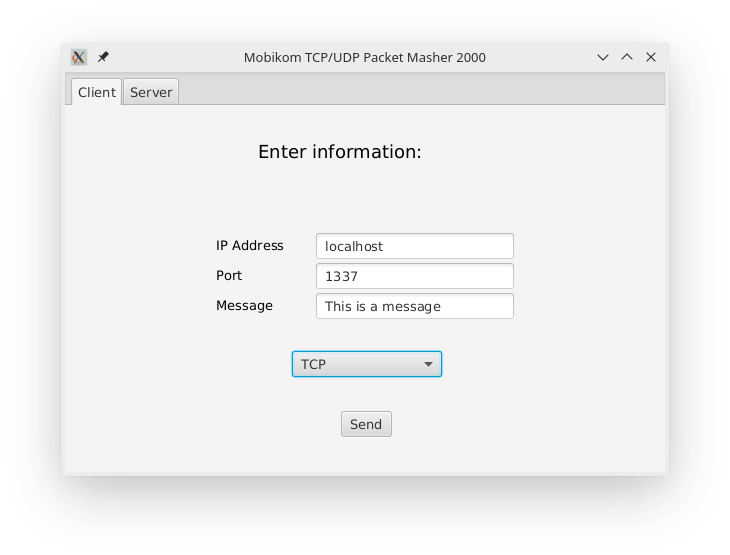
\includegraphics[width=1.1\linewidth]{images/task1/client.png}
		\caption{The client interface with JavaFX}
		\label{fig:clientfx}
	\end{subfigure}%
	\begin{subfigure}{.49\textwidth}
		\centering
		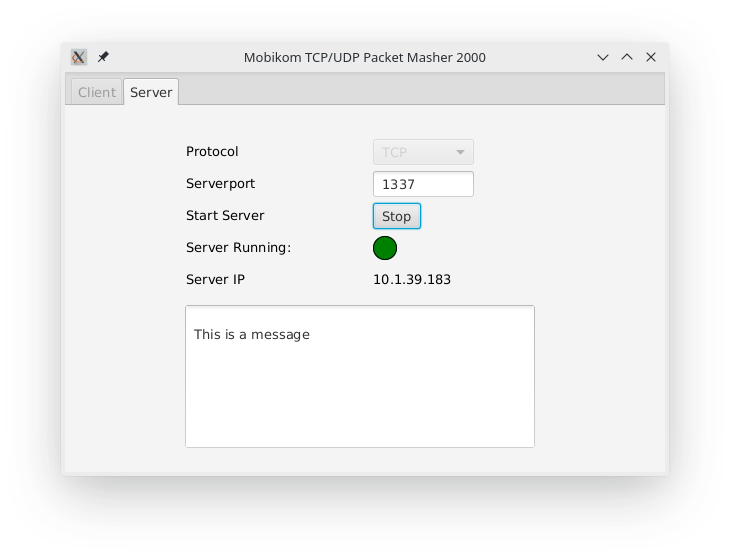
\includegraphics[width=1.1\linewidth]{images/task1/server.png}
		\caption{The server interface with JavaFX}
		\label{fig:serverfx}
	\end{subfigure}
	\caption{The Desktop application, structured with tabs.}
	\label{fig:fx}
\end{figure}

\begin{figure}[H]
	\centering
	\begin{subfigure}{.49\textwidth}
		\centering
		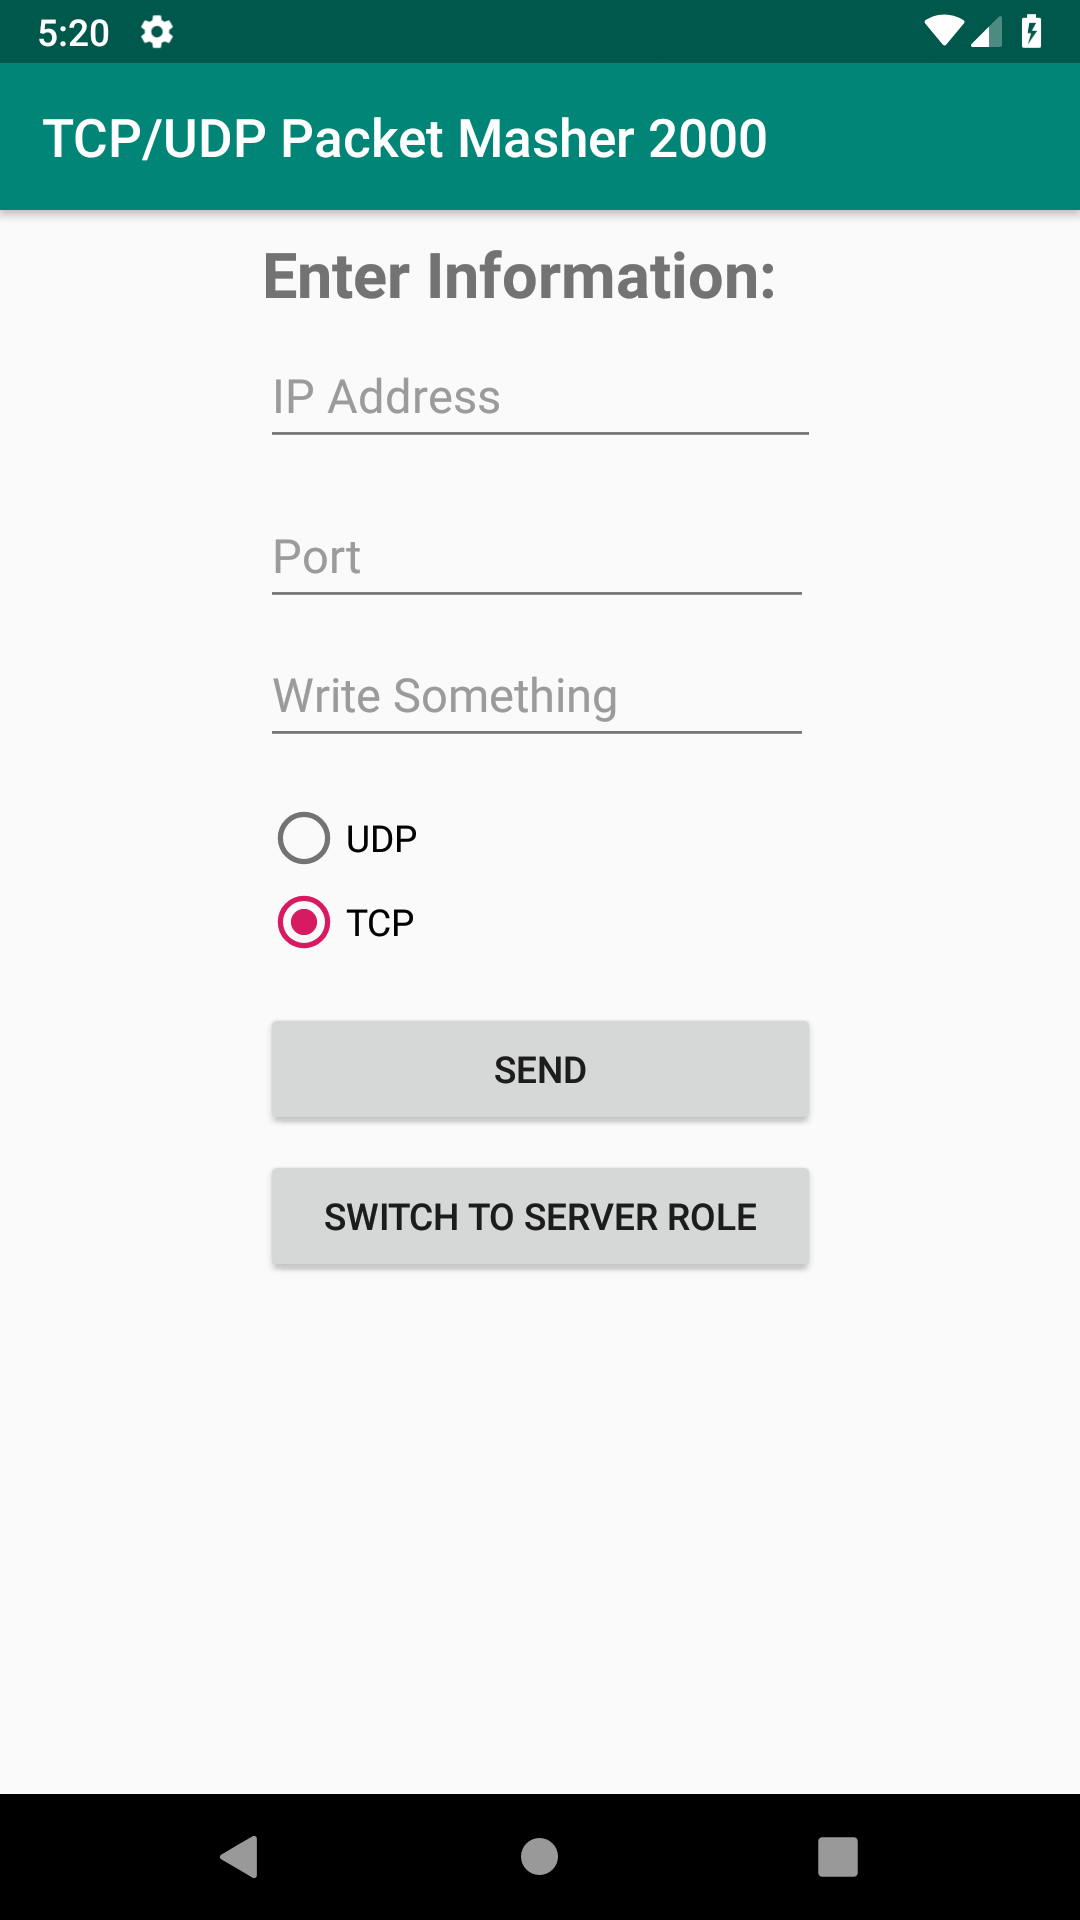
\includegraphics[width=0.75\linewidth]{images/task1/clientAndroid.png}
		\caption{The client activity on Android}
		\label{fig:clientAndroid}
	\end{subfigure}%
	\begin{subfigure}{.49\textwidth}
		\centering
		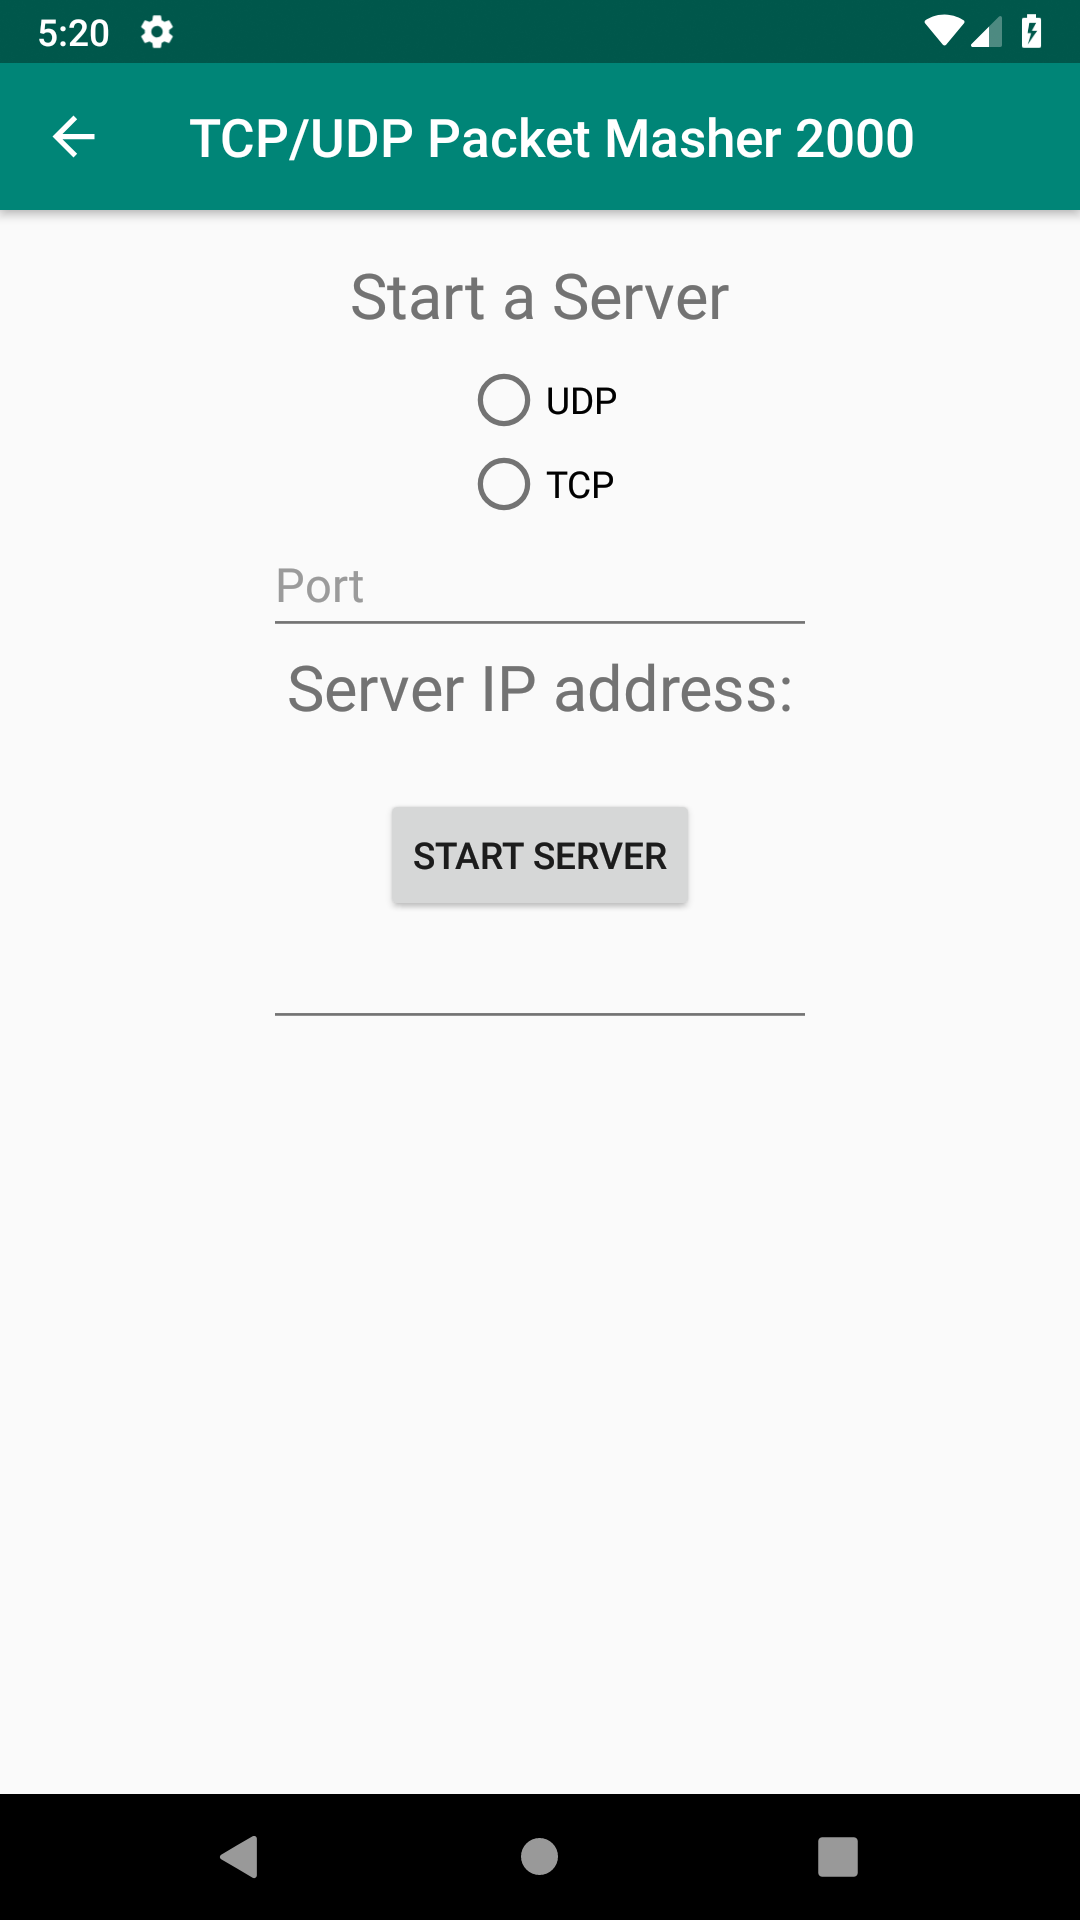
\includegraphics[width=0.75\linewidth]{images/task1/serverAndroid.png}
		\caption{The server activity on Android}
		\label{fig:serverAndroid}
	\end{subfigure}
	\caption{The Android application, structured with two activities}
	\label{fig:android}
\end{figure}

The screenshots provided in figure \ref{fig:fx} provide an overview of the graphical user interface written for the Desktop or JVM application which  is written with the help of JavaFX. 

Figure \ref{fig:android} summarizes the user interface specific to the Android application. 



\subsection{Implementation of a TCP Client}

The program employs an MVC pattern, separating the source code in three parts: model, view and control. The networking part of the code is bundled in the \textit{communication} package, where the rest of the program only interacts with the \textit{Communicator} class. The strategy pattern is applied at this point which allows to seamlessly switch between underlying protocol, namely TCP and UDP. The functionalities of each of the protocols are bundled in a class implementing the \textit{Connector} interface. This ensures that each of the protocol specific implementations offers the needed operations. In the case of the client, the interface specifies a contract where the method \textit{sendMessage} has to be realized as can be seen in \ref{lst:sendMessageI}.

\begin{lstlisting}[language=Java, caption={Interface prescribes a sendMessage method},captionpos=b,label=lst:sendMessageI]
/**
 * Sends message to specified ip-address:port.
 *
 * @param ip      receiver address
 * @param port    and receiver port
 * @param message message to be transported
 */
public void sendMessage(String ip, int port, String message);
\end{lstlisting}

The implementation of the \textit{sendMessage} method for the TCP connector can be seen in listing \ref{lst:sendMessageTCP}. In order to offload this functionality into a seperate thread an \textit{ExecutorService} is used where tasks, can be submitted for execution. This ensures the user interface, running on the main thread, does not freeze even if the sending of a message or the establishing of a connection either takes a long time or is unsuccessful.

\begin{lstlisting}[language=Java, caption={TCP sendMessage implementation},captionpos=b,label=lst:sendMessageTCP]
private ExecutorService exs = Executors.newCachedThreadPool();
public void sendMessage(String ip, int port, String message) {
	logger.log(Level.INFO, "Sending message : " + message + " to: " + ip + ":" + port);
	TCPMessageTask messageTask = new TCPMessageTask(ip, port, new Message(message));
	exs.submit(messageTask);
}
\end{lstlisting}

Listing \ref{lst:TCPMessageTask} shows the implementation of the sending of a TCP message. The try-with-resource block ensures that the socket is automatically closed when reaching the end of the statement. Specifying a timeout for the connecting of the \textit{clientSocket} guarantees that after maximally 2000ms this blocking method continues in execution. Since this is executed in its own thread, the termination of the complete program depends on the termination of this method. Finally, the message that was passed as string value has been bundled in an instance of the \textit{Message} class that implements the \textit{Serializable} interface. 

\begin{minipage}{\linewidth}
	\begin{lstlisting}[language=Java, caption={TCP sendMessageTask implementation},captionpos=b,label=lst:TCPMessageTask]
@Override
public void run() {
  //try-with-resources block auto closes the socket
  try (Socket clientSocket = new Socket()) {
    InetAddress addr = InetAddress.getByName(ip)
    InetSocketAddress socketAddr = new InetSocketAddress(addr);
    clientSocket.connect(socketAddr, port), 2000);
    //Initialize an object output stream to send the message object
    try (ObjectOutputStream out = new ObjectOutputStream(clientSocket.getOutputStream())) {
      out.writeObject(message);
      out.flush();
    }
			
    } catch (IOException e ) {
      e.printStackTrace();
    }
}
	\end{lstlisting}
\end{minipage}

\subsection{Implementation of a TCP Server}

The same program will be used to start a TCP server listening for incoming connections. In order to keep the concerns separated, once a server has been started, the tab allowing for using the application as a TCP client will be disabled. The \textit{Connector} interface prescribes the implementation of a method that shall start a server (see listing \ref{startServerI}). 

\begin{lstlisting}[language=Java, caption={Interface prescribes a startServer method},captionpos=b,label=lst:startServerI]
/**
 * This method starts a server with the set protocol on specified port. The controller will be used to update the interface, especially with received messages.
 *
 * @param port       Port the server listens to
 * @param controller a controller that can be used to for instance update the GUI, display received messages
 */
public void startServer(int port, ControllerInterface controller);
\end{lstlisting}

The server implementation is again multithreaded, making use of the same \textit{ExecutorService} instance, that employs a cached thread pool. The runnable that holds the server logic in the run-method, can be seen in listing \ref{lst:runServer}. In order to be able to accept multiple connections, a while-loop checks the value of the \textit{running} boolean. The \textit{volatile} keyword makes sure that a change to this value crosses the memory barrier and the while-loop is stopped when requested. Therefore, all created tasks are stored in a list, and once shutdown is requested, the boolean of each task is set to false. The program successfully terminates.

\begin{minipage}{\linewidth}
	\begin{lstlisting}[language=Java, caption={Run method of TCPServerTask},captionpos=b,label=lst:runServer]
private volatile boolean running = true;
@Override
public void run() {
  while (running) {
	try (ServerSocket serverSocket = new ServerSocket(port)) {
		serverSocket.setSoTimeout(1000);
		try (Socket clientSocket = serverSocket.accept()) {
			...
		} catch (SocketTimeoutException ignored) {}
	} catch (IOException e) {
	 ...
	}
  }
}
	\end{lstlisting}
\end{minipage}

The communication package bundling the network specific classes was exported with the help of eclipse as a \textit{.jar} file. This file was added as a library to the Android project, ensuring a seamless reuse of the already written parts.

\begin{figure}[H]
	\centering
	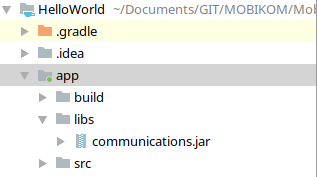
\includegraphics[width=0.5\linewidth]{images/task1/jar.png}
	\caption{Communicaions.jar in the Android project}
	\label{fig:jar}
\end{figure}